  \let\negmedspace\undefined
\let\negthickspace\undefined
\documentclass[journal]{IEEEtran}
\usepackage[a5paper, margin=10mm, onecolumn]{geometry}
\usepackage{lmodern} % Ensure lmodern is loaded for pdflatex
\usepackage{tfrupee} % Include tfrupee package

\setlength{\headheight}{1cm} % Set the height of the header box
\setlength{\headsep}{0mm}     % Set the distance between the header box and the top of the text

\usepackage{gvv-book}
\usepackage{gvv}
\usepackage{cite}
\usepackage{amsmath,amssymb,amsfonts,amsthm}
\usepackage{algorithmic}
\usepackage{graphicx}
\usepackage{textcomp}
\usepackage{xcolor}
\usepackage{txfonts}
\usepackage{listings}
\usepackage{enumitem}
\usepackage{mathtools}
\usepackage{gensymb}
\usepackage{comment}
\usepackage[breaklinks=true]{hyperref}
\usepackage{tkz-euclide} 
\usepackage{listings}                                      
\def\inputGnumericTable{}                                 
\usepackage[latin1]{inputenc}                                
\usepackage{color}                                            
\usepackage{array}                                            
\usepackage{longtable}
\usepackage{multicol}
\usepackage{calc}                                             
\usepackage{multirow}                                         
\usepackage{hhline}                                           
\usepackage{ifthen}                                           
\usepackage{lscape}
\begin{document}
	
	\bibliographystyle{IEEEtran}
	\vspace{3cm}
	
	\title{9.5.7}
	\author{EE24BTECH11059 - Y Siddhanth}
	% \maketitle
	% \newpage
	% \bigskip
	{\let\newpage\relax\maketitle}
	
	\renewcommand{\thefigure}{\theenumi}
	\renewcommand{\thetable}{\theenumi}
	\setlength{\intextsep}{10pt} % Space between text and floats
	
	
	\numberwithin{equation}{enumi}
	\numberwithin{figure}{enumi}
	\renewcommand{\thetable}{\theenumi}
	
	
	\textbf{Question}:\newline
	Solve the below differential equation such that the function passes through $\brak{1,1}$.\[
	\left\{ x \cos\left(\frac{y}{x}\right) + y \sin\left(\frac{y}{x}\right) \right\} y \, dx = 
	\left\{ y \sin\left(\frac{y}{x}\right) - x \cos\left(\frac{y}{x}\right) \right\} x \, dy
	\]
	\textbf{Solution: }\\
	Theoretical Solution:
	\begin{align}
		\left\{ x \cos\left(\frac{y}{x}\right) + y \sin\left(\frac{y}{x}\right) \right\} y \, dx &= 
		\left\{ y \sin\left(\frac{y}{x}\right) - x \cos\left(\frac{y}{x}\right) \right\} x \, dy \\ 
		\frac{dy}{dx} &= \frac{ \brak{x \cos\left(\frac{y}{x}\right) + y \sin\left(\frac{y}{x}\right) }y}{\brak{y \sin\left(\frac{y}{x}\right) - x \cos\left(\frac{y}{x}\right) }x} \\
		\frac{dy}{dx} &= \frac{ \brak{x \cos\left(\frac{y}{x}\right) + y \sin\left(\frac{y}{x}\right) }y}{\brak{y \sin\left(\frac{y}{x}\right) - x \cos\left(\frac{y}{x}\right) }x}
	\end{align}
	Taking $v = \frac{y}{x} \implies \frac{dy}{dx} = v + x\frac{dv}{dx}$ and simplifying
	
	\begin{align}
		\frac{dy}{dx} &= \frac{ \brak{1 + v \tan\brak{x} }v}{\brak{v \tan\brak{v} - 1 }}\\
		v + x\frac{dv}{dx} &= \frac{ \brak{1 + v \tan\brak{x} }v}{\brak{v \tan\brak{v} - 1 }}\\
		x\frac{dv}{dx} &= \frac{ 2v}{\brak{v \tan\brak{v} - 1 }}\\
		2\int\frac{dx}{x} &=  \int\tan\brak{v}dv - \int\frac{dv}{v}
	\end{align}
	Solving the integral, we get
	\begin{align}
		2\log\brak{x} + \log{\brak{v}} &= \log|sec{\brak{v}|} + c \\
		2\log\brak{x} + \log{\brak{\frac{y}{x}}} &= \log\abs{sec{\brak{\frac{y}{x}}}} + c \\
		\log{\brak{xy\abs{\cos\brak{\frac{y}{x}}}}} &= c\\
	\end{align}
	Substituting the given conditions,
	\begin{align}
		e^c &= 0.54
	\end{align}
	The theoretical solution is,
	\begin{align}
		xy\abs{\cos\brak{\frac{y}{x}}} &= 0.54\\
	\end{align}
	\newline
	Numerical Solution:\newline
	The numerical solution for this differential equation can be found using the method of Finite Differences \eqref{finited} involving multiple varied stepsizes, bounded (x,y) coordinates and bounded derivative value.
	\begin{align}
		\frac{dy}{dx} &= \frac{y\brak{x+h} - y\brak{x}}{h} \\
		\implies y\brak{x+h} &= y\brak{x} + h\cdot\frac{dy}{dx} \label{finited}
	\end{align}
	Substituting $\frac{dy}{dx}$ into \eqref{finited}, we get
	\begin{align}
		\implies y(x+h) &= y(x) + h\cdot\frac{ \brak{x \cos\left(\frac{y}{x}\right) + y \sin\left(\frac{y}{x}\right) }y}{\brak{y \sin\left(\frac{y}{x}\right) - x \cos\left(\frac{y}{x}\right) }x} 
	\end{align}
	By using this method iteratively $\brak{x \implies x_n \text{ and } x+h \implies x_{n+1}}$, we can numerically find all the points lying on the curve. The accuracy can be controlled by varying the stepsize or $h$.
	\begin{align}
		y(x_{n+1}) &= y(x_n) + h\cdot\frac{ \brak{x_n \cos\left(\frac{y_n}{x_n}\right) + y_n \sin\left(\frac{y_n}{x_n}\right) }y_n}{\brak{y_n \sin\left(\frac{y_n}{x_n}\right) - x_n \cos\left(\frac{y_n}{x_n}\right) }x_n} 
	\end{align}
	However, this method, with a single step, fails to plot the entire curve when there are multiple branches, discontinuities, or infinite gradients. In this specific problem, the plot consists of an infinite number of skewed hyperbolas, which are impossible to capture using the simple finite differences method.  
	
	This limitation can be addressed by employing multiple step sizes. A large step is initially taken from \(x_0 \to x_1\) (\(h_1\)), and then the points between them are filled using smaller steps (\(h_2 = 0.01\)) in both forward and backward directions. The large steps are taken in a backward direction, where points approach the origin, with step sizes varying from \(0.1 \to 1\), incremented by \(0.001\). Finally, a gradient limit is introduced to avoid infinite gradients and stationary points.  
	
	While this approach has limitations near the \(x\)-axis due to the varying large steps approaching the origin, it performs well as the distance from the origin increases.
	
	\begin{figure}[h!]
		\centering
		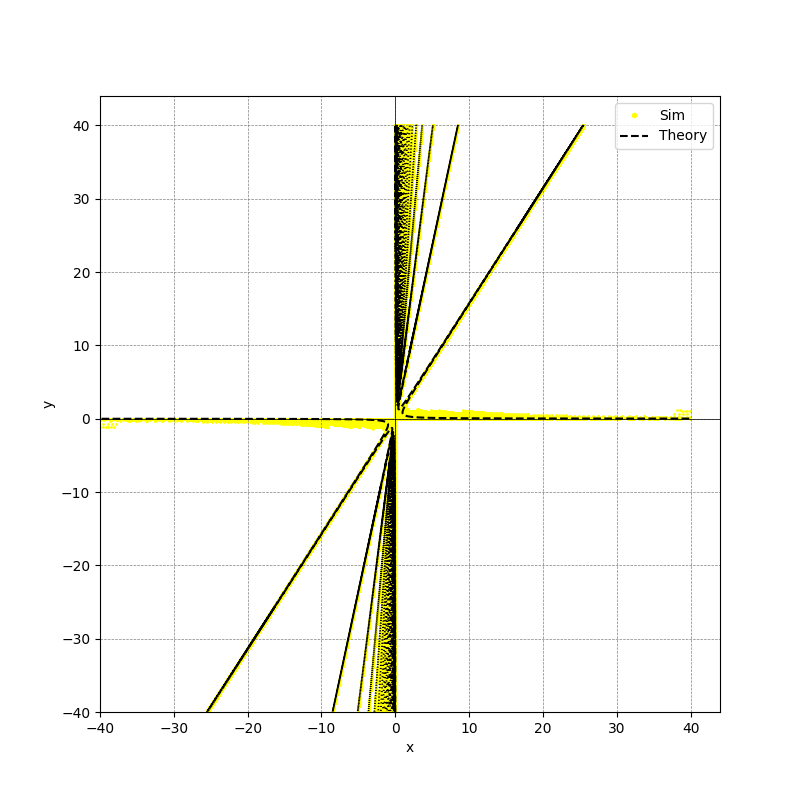
\includegraphics[width=\columnwidth]{figs/fig1.png}
		\caption{Comparison between the Theoretical solution and Numerical solution}
		\label{stemplot}
	\end{figure}
\end{document}  